%Se podrá presentar en dos Capítulos separados: Capítulo 4: Resultados y Capítulo 5: Discusión

%HIPÓTESIS: la linealidad se mantiene o no con la escala

\section {Bloque/Núcleo 1-A1-Propuesta de relevamiento por imágenes RGB de las reservas de la provincia de Misiones}
%Comenzaría por una descripción territorial de las reservas, proponiendo una clasificación, que puede ser por público o privada, ubicación, superficie, etc. Luego vendría una propuesta de las opciones: satelital, aérea tripulada y aérea no tripulada, restringiendonos a imágenes RGB. Acompaña a cada opción un análisis técnico económico. Finalmente, concluir con cuál sería la mejor opción dependiendo del tipo de reserva y la resolución pretendida. Brindar una herramienta de toma de decisión para quien desee hacer un relevamiento de reservas en la provincia de Misiones.
El propósito de esta sección es realizar un análisis comparativo del relevamiento entre distintas áreas de reservas forestales. Se consideran casos extremos en extensión grande como es la reserva Biósfera Yaboty, de más de 250 mil hectáreas, y por otro lado se analizan algunas reservas públicas o privadas de alrededor de pocas hectáreas de extensión. El objetivo es obtener herramientas que faciliten la toma de decisiones sobre la estrategia adecuada para el relevamiento y monitoreo forestal, tanto en el ámbito público como el privado, en la provincia de Misiones. Los parámetros que son considerados para el análisis son el tiempo que implica la captura de imágenes, la necesidad de recursos para almacenamiento, requerimientos económicos y restricciones legales y reglamentarias.


\section{ Propuesta de Herramientas de Bajo Costo (Económico y Computacional) para el relevamiento del bosque atlántico}
\subsection{A2-Relación de iluminación natural con histogramas de color}
Con el objeto de evaluar la correspondiente afectación en el histograma de las imágenes capturadas respecto a las condiciones de iluminación natural, se hicieron varias capturas en distintos horarios durante varios días desde una posición fija a un determinado objeto (un árbol de palta) y se midió la iluminancia usando un luxómetro.
\subsection{B-Replicación del paper de Wagner}
A partir de un trabajo publicado por \cite{hubert_wagner_individual_2018}, se intentó replicar una parte del mismo que implementaba una serie de procedimientos morfológicos a una imagen aérea o satelital en escala de grises de una porción de selva, para delinear copas individuales previo a realizar una clasificación de especies.

3 Evaluación de la influencia de diferentes parámetros en los 
algoritmos
Se evaluó el desempeño de los algoritmos modificando en un determinado rango el
valor de distintos parámetros en cada etapa del procesamiento, para observar en qué
modo se ven afectados los resultados. Se procedió a lo que se denomina “Gridsearch”,
estableciendo valores de parámetros en grillas y los correspondientes resultados delprocesamiento de las imágenes. En este procedimiento se evidencia la importancia y la
vinculación que tienen los parámetros en las diferentes etapas con la resolución espacial
de la imagen con la que se trabaja. En tanto en la última etapa se observó que el umbral
que se definió para separar (y por lo tanto binarizar la imagen) las copas segmentadas,
en el artículo de referencia sugiere utilizar el umbral del 0,001 percentil, pero al hacer la
prueba de Gridsearch con diferentes valores hasta el 0,9 percentil, resultaba notable que
excepto el correspondiente al percentil 0,9 los demás resultados no eran visiblemente
diferentes.
\subsubsection{RESULTADOS HOMOMÓRFICO}
Los resultados de las pruebas se exponen en la Tabla I. Allí se visualiza para distintas imágenes la cantidad de sombras detectadas, y se comparan los resultados de conteo automático con distintos tamaños de ventana, con el método de búsqueda de forma manual. Nótese el cambio de signo para el error medio entre los tamaños de ventana de 25 y de 20 píxeles, indicando que la selección de un tamaño de ventana menor resultará en una mayor 
cantidad de sombras detectadas que la que se obtiene por conteo manual. En cambio un tamaño de ventana mayor podría obviar varias sombras que serían tenidas en cuenta para el conteo manual. De acuerdo con la resolución de las imágenes de prueba, el tamaño de ventana cuadrada de 20 píxeles por lado se correspondería con un área de 100 metros cuadrados.




\subsubsection{Resultados IIC} \label{Resultados}
Un total de diecinueve imágenes aéreas de selva fueron consideradas para realizar el análisis. Dos de ellas representativas de los diferentes escenarios que fueron cubiertos, se muestran en las figuras \ref{calle} y \ref{tupido}. La figura \ref{calle} muestra una imagen en la que unas pocas copas de árboles se distribuyen por el área capturada, mientras que en la \ref{tupido} el dosel cubre prácticamente toda el área. La delineación manual de las sombras fue realizada como se describe en el apartado de \ref{Metodología}
Dos ejemplos de máscaras manuales se muestran en figuras \ref{contorno1} y \ref{contorno2}, con trazo rojo bordeando las regiones sombreadas. La figura \ref{superposicion} muestra el solapamiento de la máscara manual (en rojo) con la automática (en azul). En la figura \ref{p60} el valor de umbral para la máscara binaria se toma del 60º percentil de la distribución de frecuencias, mientras que en la figura \ref{p85} el valor de umbral es tomado del 85º percentil.

\begin{figure}
    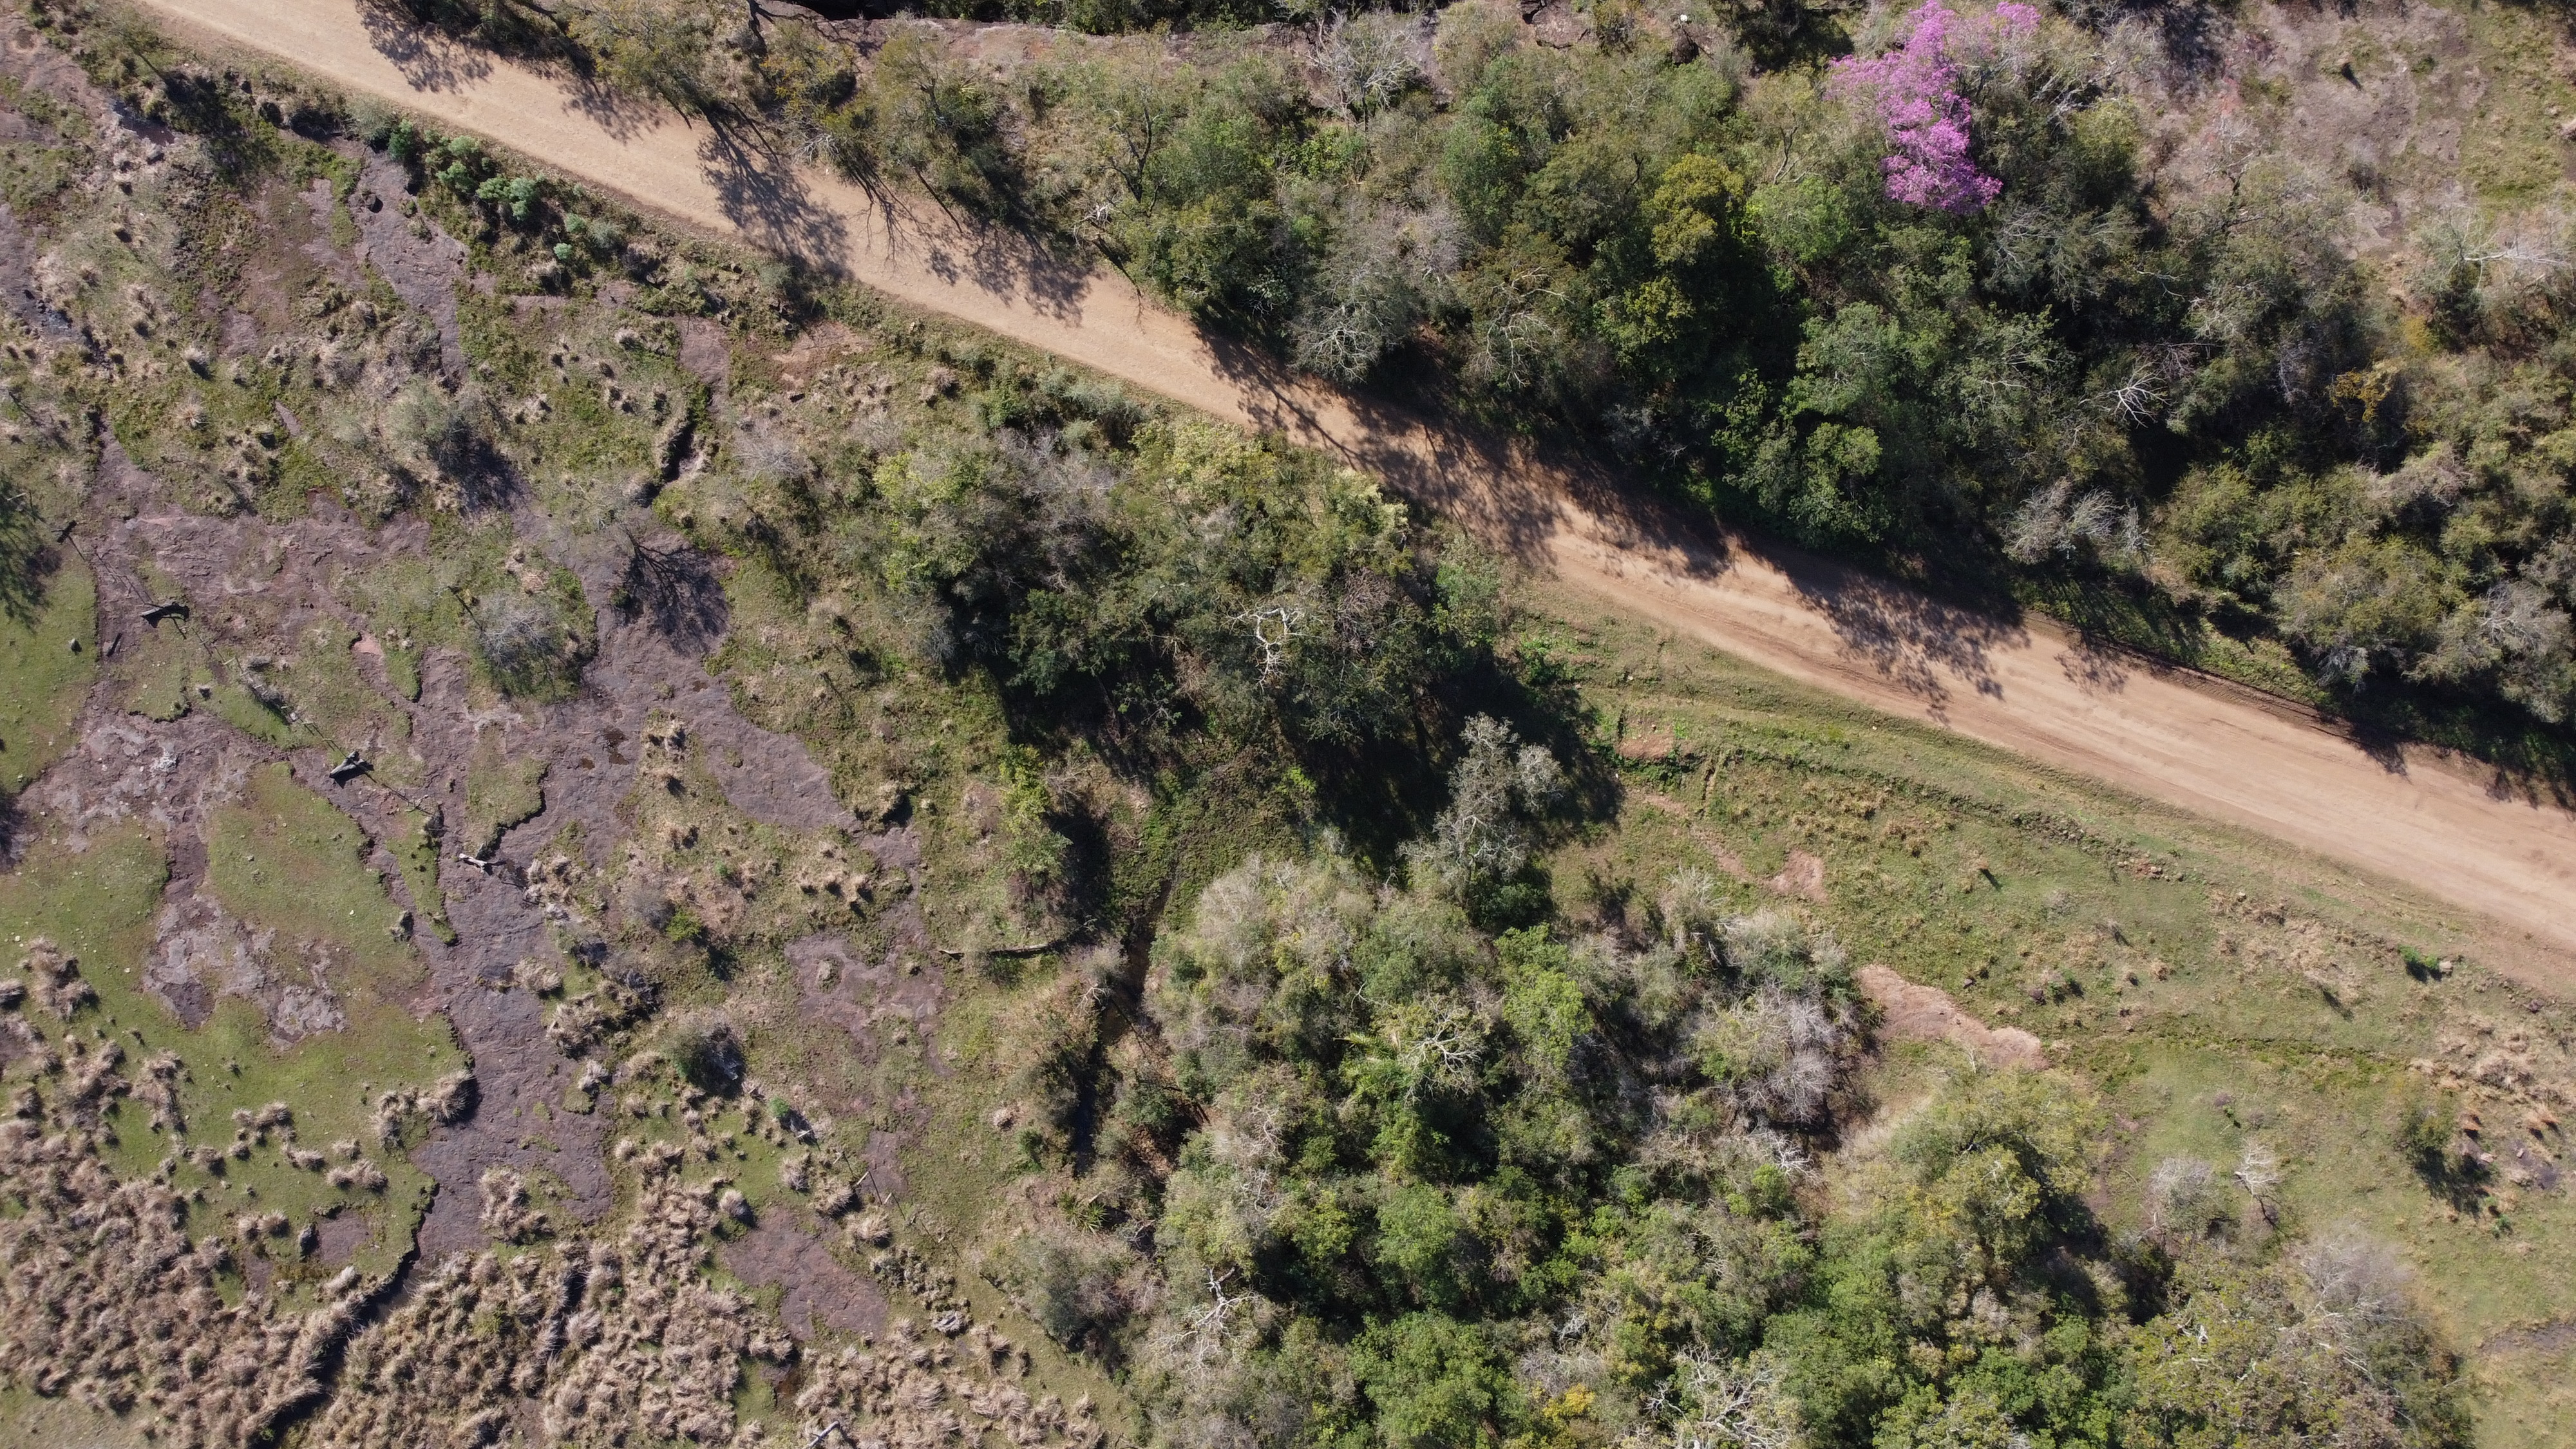
\includegraphics[width=\textwidth]{Imagenes/street.jpg}
     \hfill
     \caption{Escena capturada con pocos árboles}
    \label{calle}
\end{figure}

\begin{figure}
    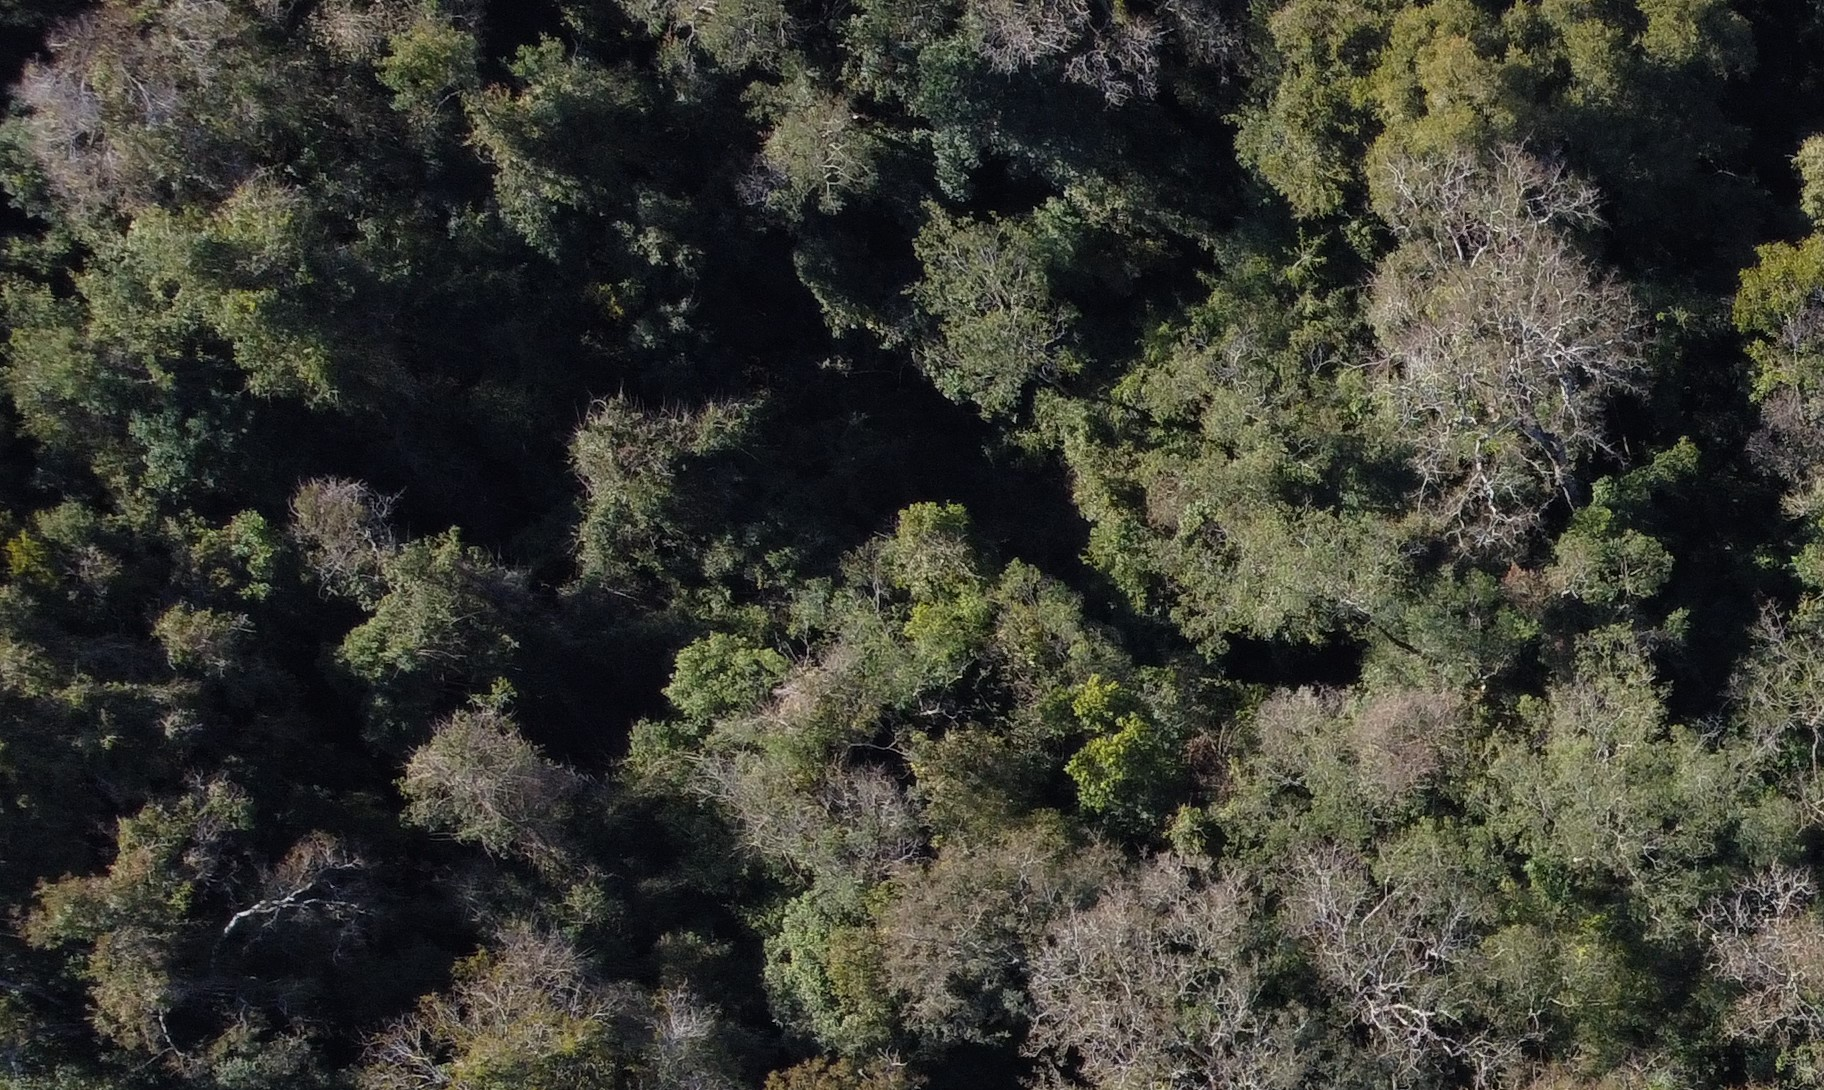
\includegraphics[width=\textwidth]{Imagenes/dense canopy.jpg}
     \hfill
     \caption{Escena capturada con dosel tupido}
    \label{tupido}
\end{figure}


\begin{figure}
    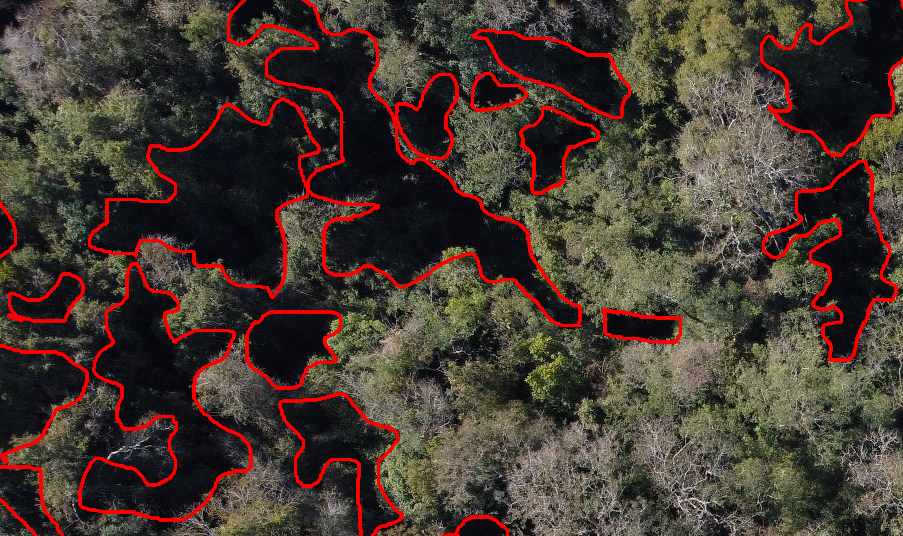
\includegraphics[width=\textwidth]{Imagenes/contours.png}
     \hfill
     \caption{Contornos de sombras en dosel tupido}
    \label{contorno1}
\end{figure}

\begin{figure}
    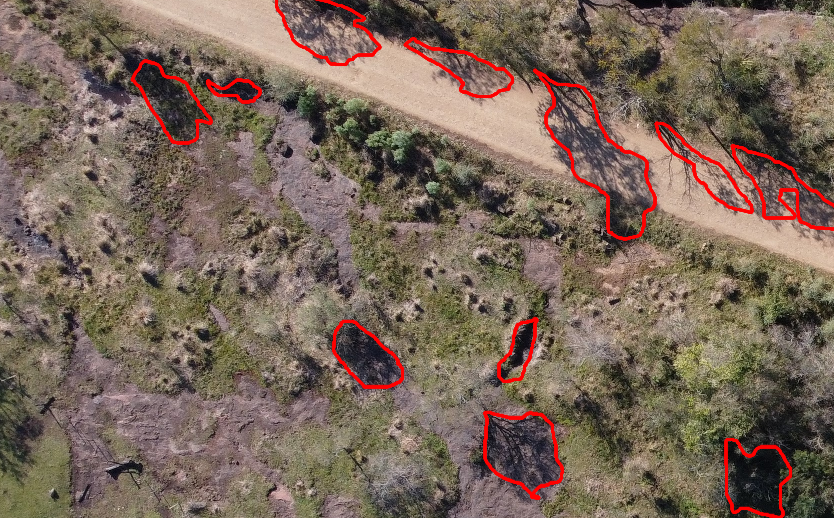
\includegraphics[width=\textwidth]{Imagenes/contours2.png}
     \hfill
     \caption{Contorno de sombras en imagen con pocos árboles}
    \label{contorno2}
\end{figure}

\begin{figure}
     \centering
     \begin{subfigure}[b]{0.5\textwidth}
         \centering
         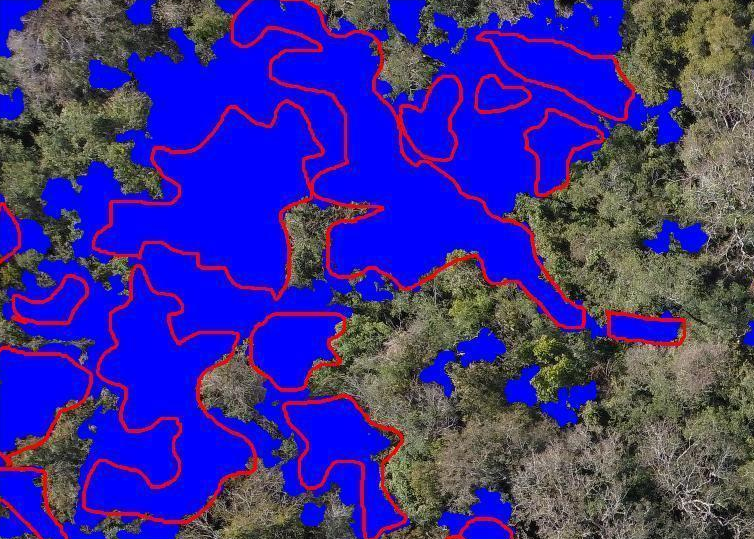
\includegraphics[width=\textwidth]{Imagenes/superposition of masks.png}
         \caption{Percentil 60º}
         \label{p60}
     \end{subfigure}
     \hfill
     
     \begin{subfigure}[b]{0.5\textwidth}
         \centering
         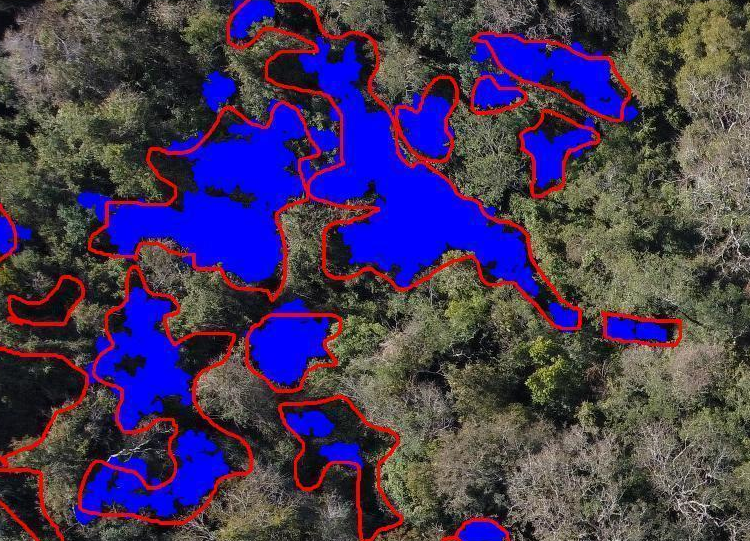
\includegraphics[width=\textwidth]{Imagenes/superposition of masks 2.png}
         \caption{Percentil 85º}
         \label{p85}
     \end{subfigure}
        \caption{Superposición de máscaras atuomática y manual}
        \label{superposicion}
\end{figure}

\begin{figure}
    \centering
  \begin{subfigure}[b]{0.3\textwidth}
    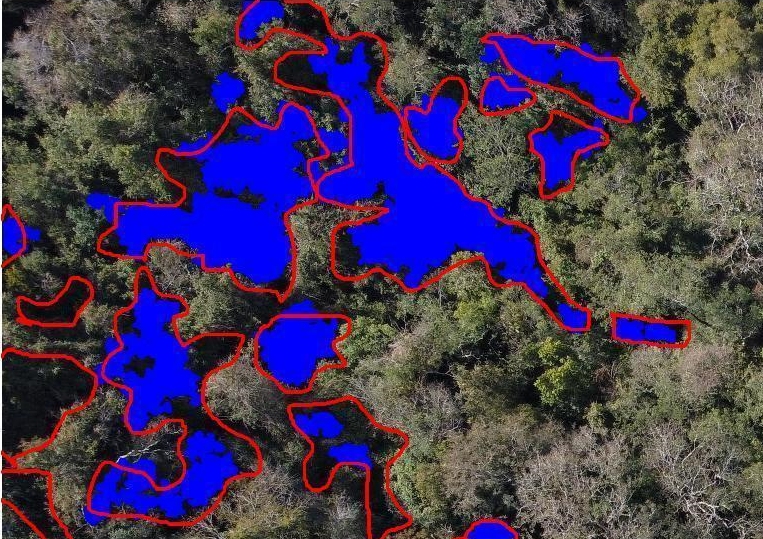
\includegraphics[width=\textwidth]{Imagenes/blue minus red 85.png}
     \hfill
     \caption{\textpsi\textsubscript{BR}}
    \label{azulrojo}
 \end{subfigure}

 \begin{subfigure}[b]{0.3\textwidth}
    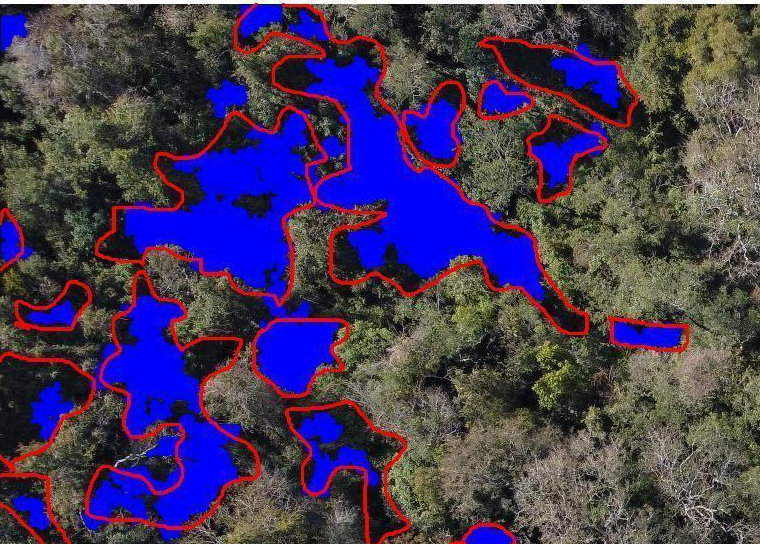
\includegraphics[width=\textwidth]{Imagenes/blue minus green 85.png}
     \hfill
     \caption{\textpsi\textsubscript{BG}}
    \label{azulverde}
 \end{subfigure}

 \begin{subfigure}[b]{0.3\textwidth}
    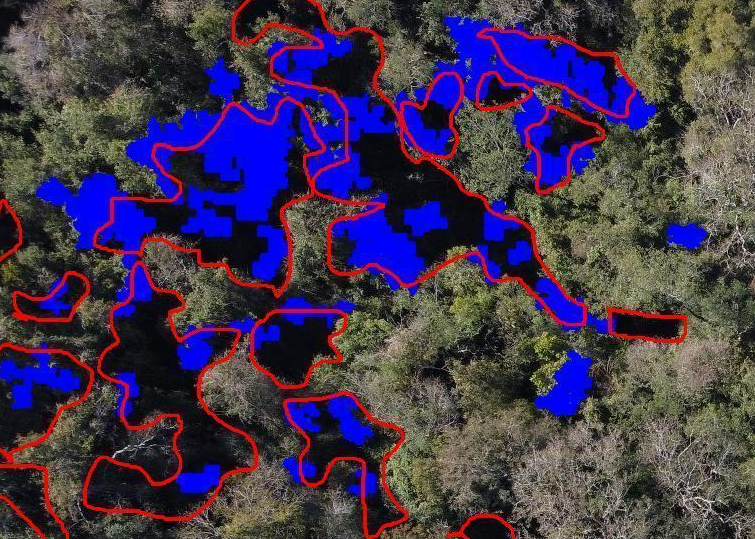
\includegraphics[width=\textwidth]{Imagenes/green minus red 85.png}
     \hfill
     \caption{\textpsi\textsubscript{GR}}
    \label{verderojo}
 \end{subfigure}
 \caption{Superposición de máscaras atuomática y manual}
        \label{p85BRBGGR}
\end{figure}

\paragraph{Influencia del valor de percentil y del índice invariante de color}

La figura \ref{azulrojo}, \ref{azulverde} y \ref{verderojo} muestra para la misma escena, diferentes máscaras automáticas obtenidas con diferentes configuraciones de la ecuación \ref{eq1}, usando tres diferentes combinaciones de canales de dos colores. La figura \ref{azulrojo} corresponde a la máscara obtenida usando la diferencia entre el canal azul menos el canal rojo $\Psi_{BR}$, la figura \ref{azulverde} usando la diferencia entre el canal azul menos el canal verde $\Psi_{BG}$ y la figura \ref{verderojo} usando la diferencia entre el canal verde menos el canal rojo $\Psi_{GR}$. En todos los casos el valor de umbral fue tomado del 85º percentil de la distribución de frecuencia. El análisis de las figuras \ref{azulrojo} a \ref{verderojo} muestra que, aplicando la ecuación \ref{eq1} usando ya sea la combinación de canales azul con verde $\Psi_{BG}$ o azul con rojo $\Psi_{BR}$  las máscaras automáticas resultantes para un mismo valor de percentil son de área mayor que las que corresponden al índice calculado con la diferencia entre canal verde y rojo $\Psi_{GR}$, lo que resulta en valores de QI más altos para $\Psi_{BR}$ y $\Psi_{BG}$ que para $\Psi_{GR}$. La comparación entre las distintas influencias del valor de percentil puede observarse en la figura \ref{curvas_QI}, donde resulta evidente que $QI_1$ es el más alto en el percentil bajo 60º y $QI_2$ es el más alto para el percentil alto 95º. Por otro lado el índice $QI_3$ se asemeja a una curva convexa, con valores similares a $QI_1$ para el percentil 60º y similares a $QI_2$ para el percentil 95º, cuyo valor máximo en la curva corresponde al 85º percentil. Un comportamiento similar se observa para los otros índices invariantes de color $\Psi_{BG}$ y $\Psi_{GR}$. La similitud entre QI1 y QI2 en el percentil más bajo se debe al hecho de que la máscara automática selecciona un área de sombra que resulta preponderante en la operación de unión binaria en el denominador de la ecuación \ref{qi3} en el caso de $QI_3$.
Por otro lado, el índice $QI_3$ se aproxima a $QI_1$ cuando la máscara automática selecciona un área pequeña de sombra, por lo tanto la selección manual de sombra resulta dominante en la operación de unión de máscaras en el denominador de la ecuación \ref{qi3}.
Al maximizar la intersección, se asegura la coincidencia entre las máscaras manual y automática, pero podría excederse en la máscara automática. Luego, al minimizar la unión, se puede controlar el tamaño pleno de la máscara automática. Un punto óptimo es el caso en el que el índice $QI_3$ alcanza el máximo valor. A pesar de la dispersión de los datos (ver figura \ref{curvas_QI}), se puede analizar los valores medios de los índices de calidad QI para los tres casos considerados (ver figuras \ref{psiBR}, \ref{psiBG}, \ref{psiGR}). Se observa que el valor que corresponde al 85º percentil de la distribución de frecuencia del índice invariante de color es el óptimo, ya que corresponde a un máximo del índice $QI_3$.
En el análisis e la figura \ref{}, se observan grandes similitudes, donde se grafican las relaciones entre los tres índices de calidad propuestos y un índice adicional definido como la diferencia entre el valor máximo y el mínimo entre los tres índices en función del valor de percentil usado para calcular el umbral de la máscara binaria automática. En los tres casos se detecta un valor mínimo para la curva que corresponde al índice adicional, es decir el rango (max - min), y este valor mínimo corresponde al percentil 85º. Además para los casos que usan sendas combinaciones en la ecuación \ref{eq1} resta de canal azul menos rojo y azul menos verde, la curva del índice $QI_3$ alcanza un valor máximo en el que corresponde al 85º percentil, mientras que este punto máximo no se hace evidente para el caso de de la combinación verde menos rojo. Por lo tanto de los cuatro índices que fueron analizados, el más conveniente es el $QI_3$, que exhibe un valor óptimo de percentil más preciso por medio del mínimo en la curva, y en los tres casos de combinaciones de canales es coincidente.

\paragraph{Influencia del filtro de mediana en la detección automática de sombras}

La figura \ref{}, \ref{} y \ref{} muestra cómo los índices que son obtenidos por las ecuaciones \ref{qi5} a \ref{qi7} son afectados por la implementación del filtro de mediana a cada imagen. En el caso del filtro de 3 x 3 píxeles, que tiene menor incidencia en los índices, los índices de calidad tienen valores mayores al 85\% para todas las imágenes. El peor desempeño lo tiene el filtro de 12 x 12, cuyo resultado comparado con la máscara automática obtenida sin filtro arrojaba una coincidencia de poco más que el 70\%.

\paragraph{Evaluación humana de máscaras automáticas de sombra}

En este trabajo los resultados del algoritmo se comparan con la selección manual llevada a cabo por expertos. Partiendo de que no hay una base de certeza absoluta (los expertos son personas humanas y por lo tanto proclives a errores de omisión o comisión), existe una limitación en el índice de calidad que se basa en este aspecto. El criterio para la selección manual de parte de los expertos depende de su particular percepción de la imagen, variando según el contexto. Por otro lado el algoritmo se basa en el cálculo de un índice y la definición de un valor umbral, obtenido de una serie de experimentos con imágenes de un determinado tipo. En otros contextos con otro tipo de imágenes el valor de umbral no sería el mismo, incluso la combinación de bandas usadas en la ecuación \ref{eq1} para obtener el índice sería diferente.
Luego de generar un conjunto de máscaras correspondientes a cada uno de los seis percentiles usando los tres índices invariantes de color de las ecuaciones \ref{psibr} a \ref{psigr} para las 19 imágenes seleccionadas, las 342 máscaras resultantes fueron comparadas con las obtenidas manualmente. Superponiendo ambas, la máscara automática y la manual sobre la imagen original, se evaluó la calidad de las similitudes mutuas, asignando un calificativo en tres niveles, "bueno", "regular" y "malo". Los resultados se muestran en la tabla \ref{tablita} y en la figura \ref{}. Tal como se puede apreciar, para los tres índices invariantes de color se puede observar un mínimo en el nivel "malo" alrededor del percentil 90º. Para los niveles "regular" y "bueno", sin embargo, el mínimo no es tan claro, lo cual puede ser atribuido a cierta subjetividad de los observadores expertos.

%%%%%%%%%%%%%%%%%%%%%%%%%%%%%%%%%%%%%%%%% TABLA %%%%%%%%%%%%%%%%%%%%%%%%%%%%%%%%%%%%%%%%%%%%%%%%%%%%%%%%%
\begin{table}[H]
    \centering
    \caption{Evaluation of the superposition of both masks. the manual and the automatic. carried on by the group of experts}
    \begin{tabular}{|c|c|c|c|c|c|c|c|}
       \hline
        COLOR INVARIANT INDEX & \multicolumn{6}{ |c|}{\textpsi \textsubscript{BR}}\\%\multicolumn{6}{ }{ |c|} \\
        \hline
        PERCENTILE & 60 & 70 & 80 & 85 & 90 & 95\\
        \hline
        GOOD & 0.0 & 0.0 & 4.5 & 15.8 & 20.5 & 0.0\\
        \hline
        REGULAR & 0.0 & 4.5 & 27.3 & 21.1 & 54.5 & 57.9\\
        \hline
        BAD & 100.0 & 95.5 & 68.2 & 63.2 & 25.0 & 42.1\\
        \hline
        COLOR INVARIANT INDEX & \multicolumn{6}{ |c|}{\textpsi \textsubscript{BG}}\\
        \hline
        PERCENTILE & 60 & 70 & 80 & 85 & 90 & 95\\
        \hline
        GOOD & 0.0 & 0.0 & 0.0 & 5.3 & 5.3 & 5.3\\
        \hline
        REGULAR & 0.0 & 5.3 & 10.5 & 15.8 & 42.1 & 21.1\\
        \hline
        BAD & 100.0 & 94.7 & 89.5 & 78.9 & 52.6 & 73.7\\
        \hline
        COLOR INVARIANT INDEX & \multicolumn{6}{|c|}{ \textpsi \textsubscript{GR}}\\
        \hline
        PERCENTILE & 60 & 70 & 80 & 85 & 90 & 95\\
        \hline
        GOOD & 0.0 & 0.0 & 0.0 & 0.0 & 0.0 & 0.0\\
        \hline
        REGULAR & 0.0 & 0.0 & 0.0 & 0.0 & 15.8 & 15.8\\
        \hline
        BAD & 100.0 & 100.0 & 100.0 & 100.0 & 84.2 & 84.2\\
        \hline
    \end{tabular}
    \\
    \raggedleft
    \label{tablita}
\end{table}
%%%%%%%%%%%%%%%%%%%%%%%%%%%%%%%%%%%%%%%%%%%%%%%%%%%%%%%%%%%%%%%%%%%%%%%%%%%%%%%%%%%%%%%%%%%%%%%%%%%%%%%%%


\begin{figure}
         \centering
         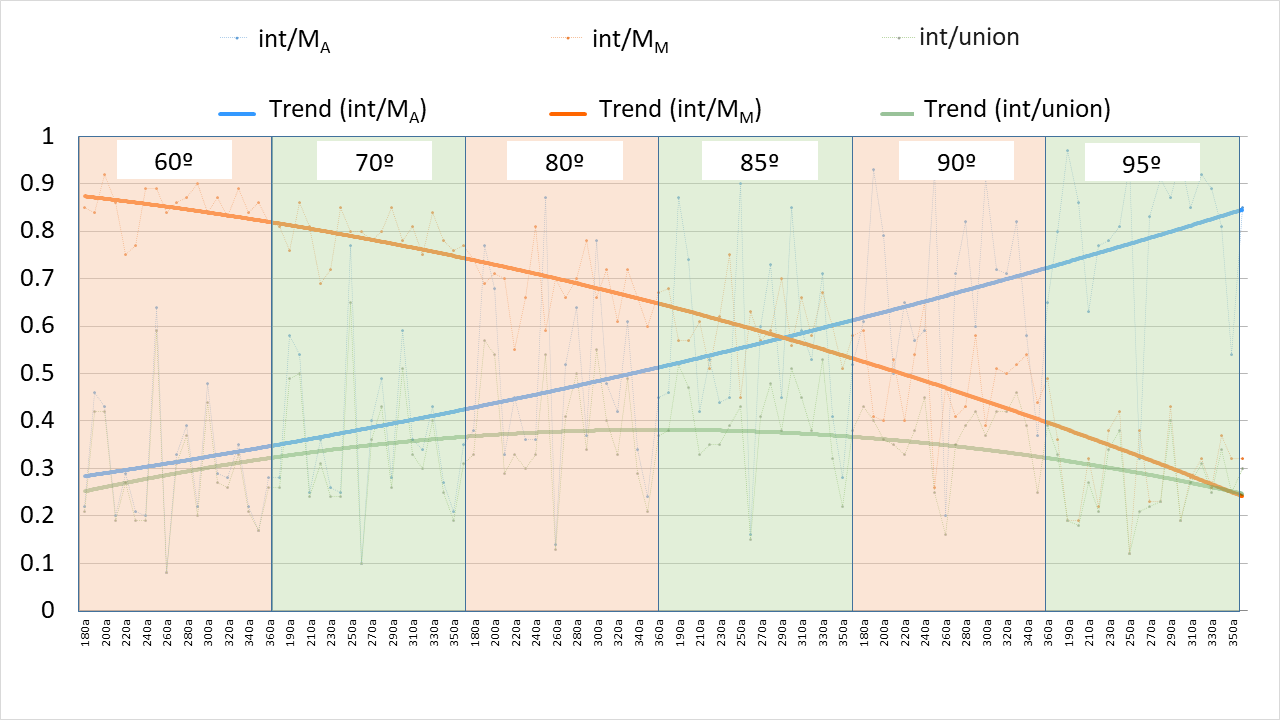
\includegraphics[width=\textwidth]{Imagenes/grafico.png}
         \hfill
         \caption{Curvas índice de calidad}
        \label{curvas_QI}
\end{figure}

%%%%%%%%%%%%%%%%%%%%%%%%%%%%%%%%%%%%%%%%%%%%%%
\begin{figure}
     \centering
     \begin{subfigure}[b]{0.3\textwidth}
         \centering
         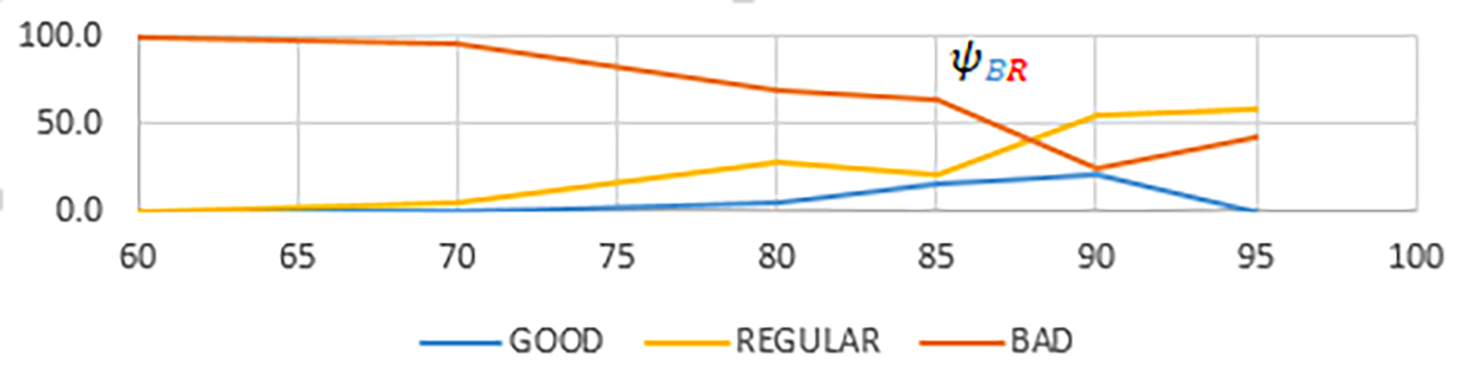
\includegraphics[width=\textwidth]{Imagenes/psiBR.png}
         \caption{\textpsi \textsubscript{BR}}
         \label{psiBR}
     \end{subfigure}
     \hfill
     \begin{subfigure}[b]{0.3\textwidth}
         \centering
         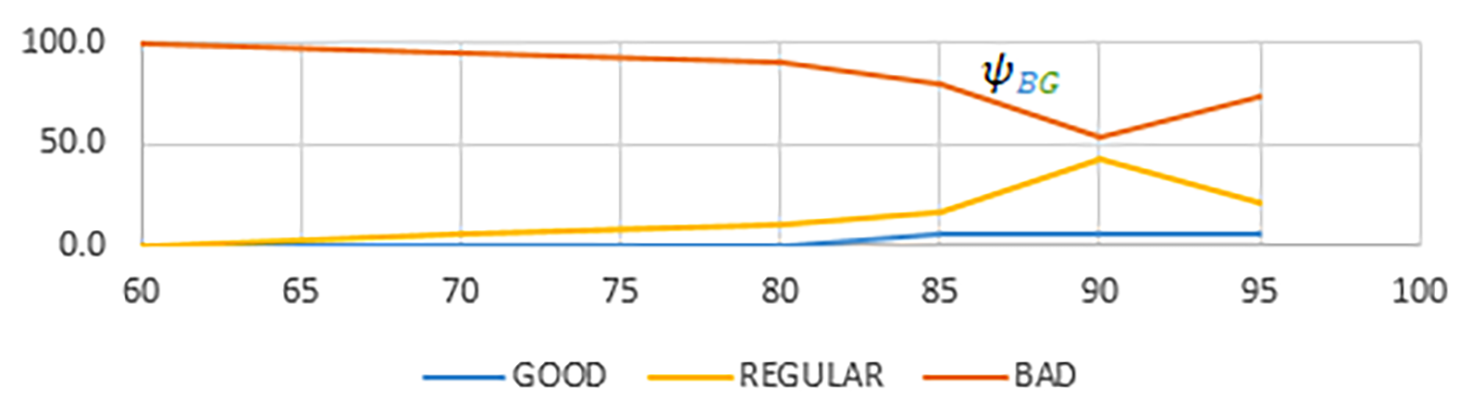
\includegraphics[width=\textwidth]{Imagenes/psiBG.png}
         \caption{\textpsi \textsubscript{BG}}
         \label{psiBG}
     \end{subfigure}
     \hfill
     \begin{subfigure}[b]{0.3\textwidth}
         \centering
         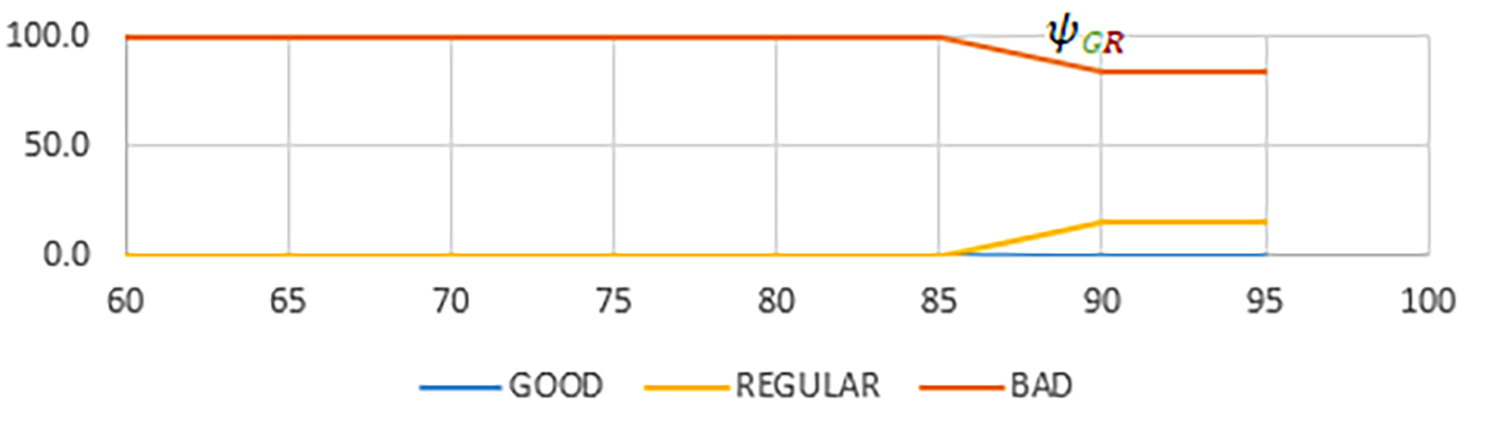
\includegraphics[width=\textwidth]{Imagenes/psiGR.png}
         \caption{\textpsi \textsubscript{GR}}
         \label{psiGR}
     \end{subfigure}
        \caption{Qualification of overlapping of both, manual and automatic masks by human experts}
        \label{humanscoring}
\end{figure}

\subsection{C3-Filtros de texturas (probados con fantomas)}
Mediante el filtrado por textura puede implementarse una segmentación o clasificación en imágenes. Se hicieron varias pruebas con imágenes simuladas (cuadrados y rombos)
\subsection{C4-Mapas autoorganizados (clasificación no supervisada)}
\subsection{C5-IIC: Análisis de efecto de bandas utilizadas (sombras)}
Informe 1
Se realizaron pruebas del algoritmo sobre distintas imágenes que contienen sombra para ver su desempeño en la selección automática de sombras. Para todos los casos se aplicó para definir el umbral de binarización el correspondiente al percentil 85 de la distribución de frecuencias del índice invariante de color calculado por la ecuación \ref{invariante de color 1}:
 %%%%%%%%%%%%%%%%%%%%%%%%%%%%%%%%%%%%%% ECUACIÓN %%%%%%%%%%%%%%%%%%%%%%%%%%%%%%%%%%%%%%%%%%%%%%%%%%%%%%%%%
\\
\begin{equation}
	\psi=\frac{4}{\pi} arctan\left(\frac{B\textsubscript{1}-B\textsubscript{2}}{B\textsubscript{1}+B\textsubscript{2}}\right),\label{invariante de color 1}
\end{equation}
\\
%%%%%%%%%%%%%%%%%%%%%%%%%%%%%%%%%%%%%%%%%%%%%%%%%%%%%%%%%%%%%%%%%%%%%%%%%%%%%%%%%%%%%%%%%%%%%%%%%%%%%%%%%
La imagen de la izquierda se procesó con la combinación de las bandas azul y verde, la de la derecha con la combinación azul y rojo.
Se observa que hay mucha similitud en las áreas marcadas, no obstante los diferentes valores de binarización, obtenidos por criterio del 85to percentil de la distribución de frecuencias de los valores de índice invariante de color hallados para cada combinación de bandas.
\\
\\
Informe 2
Aplicando el algoritmo sobre una imagen seleccionada que contiene sombras, usando la ecuación \ref{invariante de color 2} en la combinación de bandas verde y roja y sin utilizar el criterio de percentil para definir el umbral de binarización:
%%%%%%%%%%%%%%%%%%%%%%%%%%%%%%%%%%%%%% ECUACIÓN %%%%%%%%%%%%%%%%%%%%%%%%%%%%%%%%%%%%%%%%%%%%%%%%%%%%%%%%%
\\
\begin{equation}
	\psi=\frac{4}{\pi} arctan\left(\frac{B\textsubscript{1}-B\textsubscript{2}}{B\textsubscript{1}+B\textsubscript{2}}\right),\label{invariante de color2}
\end{equation}
\\
%%%%%%%%%%%%%%%%%%%%%%%%%%%%%%%%%%%%%%%%%%%%%%%%%%%%%%%%%%%%%%%%%%%%%%%%%%%%%%%%%%%%%%%%%%%%%%%%%%%%%%%%%
Observando la imagen con la máscara superpuesta en color azul se nota una marcación altamente coincidente con la que corresponde al área sombreada. Además, mediante el gráfico de histograma de frecuencias del índice invariante de color es posible advertir el valle entre dos picos situado en torno al valor 0,2 el cual fue usado como umbral de binarización.
\\
\\
Informe 3

Tal como surge de la ecuación 1, las posibilidades de combinar dos entre tres bandas de color resultan en seis diferentes índices invariantes de color para una imagen dada. Lo que resulta notorio es que a priori no se sabe cuál de esas seis resulta la más adecuada para constituir la máscara de selección automática de sombras. 

